\documentclass[letterpaper,12pt,oneside]{article}\usepackage[]{graphicx}\usepackage[]{color}
%% maxwidth is the original width if it is less than linewidth
%% otherwise use linewidth (to make sure the graphics do not exceed the margin)
\makeatletter
\def\maxwidth{ %
  \ifdim\Gin@nat@width>\linewidth
    \linewidth
  \else
    \Gin@nat@width
  \fi
}
\makeatother

\definecolor{fgcolor}{rgb}{0.345, 0.345, 0.345}
\newcommand{\hlnum}[1]{\textcolor[rgb]{0.686,0.059,0.569}{#1}}%
\newcommand{\hlstr}[1]{\textcolor[rgb]{0.192,0.494,0.8}{#1}}%
\newcommand{\hlcom}[1]{\textcolor[rgb]{0.678,0.584,0.686}{\textit{#1}}}%
\newcommand{\hlopt}[1]{\textcolor[rgb]{0,0,0}{#1}}%
\newcommand{\hlstd}[1]{\textcolor[rgb]{0.345,0.345,0.345}{#1}}%
\newcommand{\hlkwa}[1]{\textcolor[rgb]{0.161,0.373,0.58}{\textbf{#1}}}%
\newcommand{\hlkwb}[1]{\textcolor[rgb]{0.69,0.353,0.396}{#1}}%
\newcommand{\hlkwc}[1]{\textcolor[rgb]{0.333,0.667,0.333}{#1}}%
\newcommand{\hlkwd}[1]{\textcolor[rgb]{0.737,0.353,0.396}{\textbf{#1}}}%

\usepackage{framed}
\makeatletter
\newenvironment{kframe}{%
 \def\at@end@of@kframe{}%
 \ifinner\ifhmode%
  \def\at@end@of@kframe{\end{minipage}}%
  \begin{minipage}{\columnwidth}%
 \fi\fi%
 \def\FrameCommand##1{\hskip\@totalleftmargin \hskip-\fboxsep
 \colorbox{shadecolor}{##1}\hskip-\fboxsep
     % There is no \\@totalrightmargin, so:
     \hskip-\linewidth \hskip-\@totalleftmargin \hskip\columnwidth}%
 \MakeFramed {\advance\hsize-\width
   \@totalleftmargin\z@ \linewidth\hsize
   \@setminipage}}%
 {\par\unskip\endMakeFramed%
 \at@end@of@kframe}
\makeatother

\definecolor{shadecolor}{rgb}{.97, .97, .97}
\definecolor{messagecolor}{rgb}{0, 0, 0}
\definecolor{warningcolor}{rgb}{1, 0, 1}
\definecolor{errorcolor}{rgb}{1, 0, 0}
\newenvironment{knitrout}{}{} % an empty environment to be redefined in TeX

\usepackage{alltt}
\usepackage[paperwidth=8.5in,paperheight=11in,top=1in,bottom=1in,left=1in,right=1in]{geometry}
\usepackage{setspace}
\usepackage[colorlinks=true,allcolors=Blue]{hyperref}
\usepackage[usenames,dvipsnames]{xcolor}
\usepackage{indentfirst}
\usepackage{titlesec}
\usepackage{multirow}
\usepackage{booktabs}
\usepackage{graphicx}
\usepackage{verbatim}
\usepackage{rotating}
\usepackage{tabularx}
\usepackage{outlines}
\usepackage{lineno}
\usepackage{array}
\usepackage{times}
\usepackage{cleveref}
\usepackage{acronym}
\usepackage[position=t]{subfig}
\usepackage{paralist}
\usepackage[noae]{Sweave}
\usepackage{natbib}
\usepackage{array}
\usepackage{pdflscape}
\usepackage{bm}
% \usepackage{showlabels}
\bibpunct{(}{)}{,}{a}{}{,}

% page margins and section title formatting
\linespread{1.5}
\setlength{\footskip}{0.5in}
\titleformat*{\section}{\Large\bf\em}
\titleformat*{\subsection}{\singlespace\large\bf}
\titleformat*{\subsubsection}{\singlespace\normalsize\bf\em}
\titlespacing{\section}{0in}{0in}{0in}
\titlespacing{\subsection}{0in}{0in}{0in}
\titlespacing{\subsubsection}{0in}{0in}{0in}

% cleveref options
\crefname{table}{Table}{Tables}
\crefname{figure}{Fig.}{Figs.}
\renewcommand{\figurename}{Fig.}

% aliased citations
% \defcitealias{FLDEP12}{FLDEP 2012}

%acronyms
\acrodef{chla}[chl-\textit{a}]{chlorophyll \textit{a}}
\acrodef{din}[DIN]{dissolved inorganic nitrogen}
\acrodef{sfe}[SFE]{San Francisco Estuary}
\acrodef{wrtds}[WRTDS]{Weighted Regressions on Time, Discharge, and Season}

%for supplemental figures/tables
\newcommand{\beginsupplement}{%
        \setcounter{table}{0}
        \renewcommand{\thetable}{S\arabic{table}}%
        \setcounter{figure}{0}
        \renewcommand{\thefigure}{S\arabic{figure}}%
     }

%knitr options


% get the version based on commit date


% get online bib file


\IfFileExists{upquote.sty}{\usepackage{upquote}}{}
\begin{document}

\raggedbottom
\linenumbers
\raggedright
\urlstyle{same}
\setlength{\parindent}{0.5in}
\renewcommand\refname{References \vspace{12pt}}

\begin{singlespace}
\title{{\bf {\Large Four decades of water quality change in the upper San Francisco Estuary}}}
\author{
  {\bf {\normalsize Marcus W. Beck$^1$, David Senn$^2$, Phil Bresnahan$^2$, Emily Novick$^2$, James D. Hagy III$^1$,}}
  \\{\bf {\normalsize Thomas Jabusch$^2$}}
  \\\\{\textit {\normalsize $^1$USEPA National Health and Environmental Effects Research Laboratory}}
  \\{\textit {\normalsize Gulf Ecology Division, 1 Sabine Island Drive, Gulf Breeze, FL 32561}}
	\\{\textit {\normalsize Phone: 850-934-2480, Fax: 850-934-2401}}
	\\{\textit {\normalsize Emails: \href{mailto:beck.marcus@epa.gov}{beck.marcus@epa.gov}, \href{mailto:hagy.jim@epa.gov}{hagy.jim@epa.gov}}}
  \\\\{\textit {\normalsize $^2$San Francisco Estuary Institute}}
	\\{\textit {\normalsize 4911 Central Avenue, Richmond, CA 94804}}
	\\{\textit {\normalsize Phone: 510-746-7334, Fax: 510-746-7300}}
	\\{\textit {\normalsize Emails: \href{mailto:davids@sfei.org}{davids@sfei.org}, \href{mailto:philb@sfei.org}{philb@sfei.org}, \href{mailto:emilyn@sfei.org}{emilyn@sfei.org}, \href{mailto:thomasj@sfei.org}{thomasj@sfei.org}}}
  \vspace{1in} 
  \\ Version Date:   Tue Jul 19 09:56:38 2016 -0500
	}
\date{}
\maketitle
\end{singlespace}
\clearpage

\begin{abstract}
\noindent Recent methods for trend analysis have been developed that leverage the descriptive potential of long-term time series.  Combined with these methods, multi-decadal datasets of water quality in coastal systems can provide valuable opportunities to gain insights into ecosystem properties and drivers of change.  This study describes use of an estuarine adaptation of the \ac{wrtds} model to describe water quality trends over four decades in the Delta region of the \ac{sfe}. This region is a complex mosaic of inflows that are primary sources of nutrients into the larger Bay.  To date, a comprehensive evaluation of the long-term monitoring dataset at multiple stations in the Delta has not been conducted despite the importance of nutrient transport from the region for water quality in the entire bay.  The \ac{wrtds} technique is data-driven where the parameterization of the functional model changes smoothly over time following dynamic patterns of season and flow.  Water quality trends that have not been previously quantified can be described, including variation in flow-normalized concentrations, frequency occurrence of extreme events, and response to historical changes in the watershed, all of which are important needs for understanding changes in the \ac{sfe}.  Model results from multiple stations in the Delta provided novel descriptions of historical trends and relationships between key species of dissolved inorganic nitrogen (ammonium, nitrate/nitrite, total).  This variation was described in the context of varying contributions of input flows from the Sacramento and San Joaquin rivers, as well as tidal exchange with the central \ac{sfe}.  Conceptual relationships between water quality and drivers of change were used to generate and test hypotheses of mechanistic relationships using selected examples from the trend descriptions. Overall, this analysis provides an ecological and management-based understanding of historical trends in the \ac{sfe} as a means to interpret potential impacts of recent changes and expected trends in this dynamic system.  An argument is also made for more comprehensive evaluations of long-term monitoring datasets to understand relationships between response endpoints and causal mechanisms in coastal waters.
\end{abstract}
\acresetall

\section{Introduction}

\begin{enumerate}
\item How and why are trends interpreted - assessment of raw data, surrogates, various methods (kendall, GAM, WRTDS), what have been implications of using different approaches, see Kratzer USGS report http://pubs.usgs.gov/sir/2010/5228/pdf/sir20105228.pdf and data http://pubs.usgs.gov/sir/2010/5228/, need to interpret eutrophication trends in estuaries - it's confusing \citep{Cloern10}
\item WRTDS, original method \citep{Hirsch10,Hirsch15}
\item WRTDS application to Tampa Bay as test set \citep{Beck15}, further validation in Patuxent and other tidal waters \cite{Beck15b}
\item SF estuary, unique and prominent location, full story is complex (historical context and recent changes) \citep{Cloern12b}, why is the delta important (a vigorous biogeochemical reactor) \citep{Jassby00,Jassby02,Jassby08}, no one has empirically described the data in the delta using data-intensive methods

San Francisco Bay on the Pacific Coast of the United States is one of the most prominent estuaries in the western hemisphere.  Background nutrient concentrations in the Bay often exceed those associated with excessive primary production, although eutrophication events have historically been infrequent.  Recent changes in response to additional stressors (e.g., variation in freshwater inputs/withdrawals, invasive species, climate change) suggests that Bay condition has not followed historical trajectories and more subtle spatial and temporal variation could provide clues that describe underlying properties of this system.  The unique ecological and social context of the Bay, including a rich source of monitoring data from the last four decades, provides a valuable opportunity to gain insight into ecosystem properties of estuaries. 

\item Study goal and objectives
\begin{itemize}
\item Provide a description of trends - annual, seasonal, spatial, response to flow, change by analytes
\item Detailed description of selected sites in the context of conceptual relationships - 1) nonlinear or extreme quantile changes, site TBD, 2) P8 and WWTP improvements, 3) Suisun DIN, SiO2, Chla, and clams
\item What this means for understanding other systems
\end{itemize}
\end{enumerate}

\section{Methods}

\subsection{Study location and data}

The \ac{sfe}... exchange with ocean, freshwater inputs (rivers and wshed drainage), runoff variation (drought years), climate, support of natural resources, subembayments, POTW (publicly owned treatment works), nutrient loading relative to other locations
\subsection{Analysis method and application}

\begin{equation}
\ln\left(N\right) = \beta_0 + \beta_1 t + \beta_2 \ln\left(Q\right) + \beta_3 \sin\left(2\pi t\right) + \beta_4 \cos\left(2\pi t\right)
\end{equation}

nine discrete sampling stations with data from 1976 to 2012, \ac{din}, ammonium, total nitrate, effects of different flow variables

Annual, seasonal trends of flow-normalized predictions

\subsection{Case studies}
These are science questions that are relevant outside of the region.
\subsubsection{Disaggregating observed nitrogen time series}
Hypothesis: Because multiple factors influence nutrient concentrations at different times, relationships between nutrients, time, and flow/salinity are non-linear and complex, so we expect 1) annual trend independent of seasonal trend, 2) changes in seasonal amplitudes and quantile trends over time, 3) varying flow contribution, either as difference between predicted/flow-normalized results or changes in nutrient v flow scatterplots at different annual periods.
\subsubsection{Effects of wastewater treatment}
Hypothesis: Modal response of nutrient concentrations at P8 over time is result of WWTP upgrades, so we expect 1) a shift in load contributions before/after upgrade, 2) a flow-normalized annual trend at P8 to show a change concurrent with WWTP upgrades, and 3) shift in the flow/nutrient relatinship before and after upgrade related to change in load contributions. See \href{http://www.waterboards.ca.gov/centralvalley/board_decisions/adopted_orders/san_joaquin/r5-2008-0086_res.pdf}{here}
\subsubsection{Effects of biological invasions}
Hypothesis: Biological invasions by benthic filter feeders have shifted abundance and composition of phytoplankton communities in Suisun Bay, so we expect 1) decline in annual, flow-normalized chlorophyll concentrations over time coincident with increase in abundance of invaders, 2) changes in ratios of limiting nutrients (nitrogen, SiO2) suggesting different uptake rates with shift in community composition, and 3) seasonal shifts in limiting nutrients based on changes in community composition and relative abundances with seasonal succession.

\section{Results}

\subsection{Trends}

\subsection{Selected examples}

\subsubsection{Disaggregating observed nitrogen time series}

\cref{fig:dinc10}, \cref{fig:dinc10dyna}

Emphasize the information the model provides relative to the observed time series.  A distinct annual trend with a maximum in the middle of the time series is observed, with lower values at the beginning and end of the period.  The seasonal patterns generally showed that \ac{din} concentrations were highest in January with higher values at moderate to low flow rates depending on the year. Interestingly, summer and fall concentrations have showed a slight increase later in the time series (~2004-2009).  The confounding effect of flow is also very apparent such that higher flows were associated with lower concentration.  Dynaplot showed that there was always a negative assocation between the two (i.e., no modal response).  The quantile distributions showed similar trends over time in both predicted values and flow-normalized predictions, although some exceptions were observed.  In particular, high flow (1984, 2008) reduced concentrations of all quantiles but the magniutude of the effect increased at higher quantiles (i.e., the effect was disproportionate).  The opposite was observed for low flow, i.e., the ninetieth percent showed the greatest increase for low flow.     

Emphasize the summer/fall change in the 2000s, why is this?  Check \citep{Cloern07}, showed seasonal changes in early 2000s in chlorophyll (NE Pacific shifted to cool phase), is there a mechanism here with DIN? Relate to conceptual diagram.

\subsubsection{Effects of wastewater treatment}

Overall reduction in total nitrogen load was observed as a result of reduction in ammonium (\cref{fig:tracy}).  Nitrate is the primary constituent of total nitrogen after 2007.  

\subsubsection{Effects of biological invasions}

Data from \citep{Crauder16}, \citet{Jassby08} describes phytoplankton community changes in the upper estuary, including chlorophyll response to flow.  Figure 10 in \citet{Jassby08} showed that chlorophyll generally decreased with flow in 1980 but inreased with flow in 2000.

Note the decrease in Potamocorbula abundance in 2011, 2012.  These are wet years where abundance/biomass of the clams is driven down by lower salinity.  Contrased wtih the annual chlorophyll trends in the same years, the predicted values are above the flow-normalized trend suggesting an increase in chlorophyll with higher flow.  The potential mechanism is therefore a decrease in clam abundance with high flow that releases phytoplankon from filtration pressure.  This also explains the positive association of chlorophyll with flow in recent years (bottom right dynaplot). 

Further, chlorophyll trends early in the time series generally show a decrease with high flow with a distinct maximum at moderate flow.  This may suggest stratification events at moderate flow contributed to phytoplankton blooms early in the time series. Water withdrawals later in the time series could have also altered environmental conditions to reduce the frequency occurrence of stratification events.  Look into this more...

What about biomass/density relationships for Potamocorbula?  Although clam density increases throughout the period,  What about initial decrease in chlorophyll prior to clam invasion?  Is this related to water withdrawals (i.e., decrease in stratification events at moderate flow)?

\cref{fig:clmchl}, \cref{fig:d7c10trnds}, \cref{tab:d7chg}, \cref{tab:c10chg}

\section{Discussion}

What do nitrogen trends mean?  Have to interpret relative to trends in other variables.  A decrease in nitrogen or constant nitrogen does not mean nitrogen inputs have stayed the same, they might actually be increasing if nitrogen.  A change in chlorohpyll relative to change in nitrogen could be informative, and even moreso, a change in silica relative to change in chlorophyll suggests diatom biomass has changed.  However, there are mismatches in these trends that suggest other processes are at play, e.g., residence times and flow inputs, etc.  Trends in Suisun relative to trends in Delta provide an example, e.g., Suisun is decrease in chlorophyll, increase in silica, increase in nitrogen, delta is decrease in silica, increase/decrease in DIN (depending on time period/season), decrease in chlorophyll, what's going on? See Senn slide 14 (from burial?). The WRTDS model lets us at least address trends in the context of season, time, and flow.  This allows for more improved interpretion relative to observing raw data. Also explain more information by looking at ammonium, nitrative/nitrite, relative to DIN. What about other variables (light level as suspended particulate matter, temperature)?

\clearpage
\begin{singlespace}
\bibliographystyle{apalike_mine}
\bibliography{refs}
\end{singlespace}
\clearpage

\begin{figure}
\centering
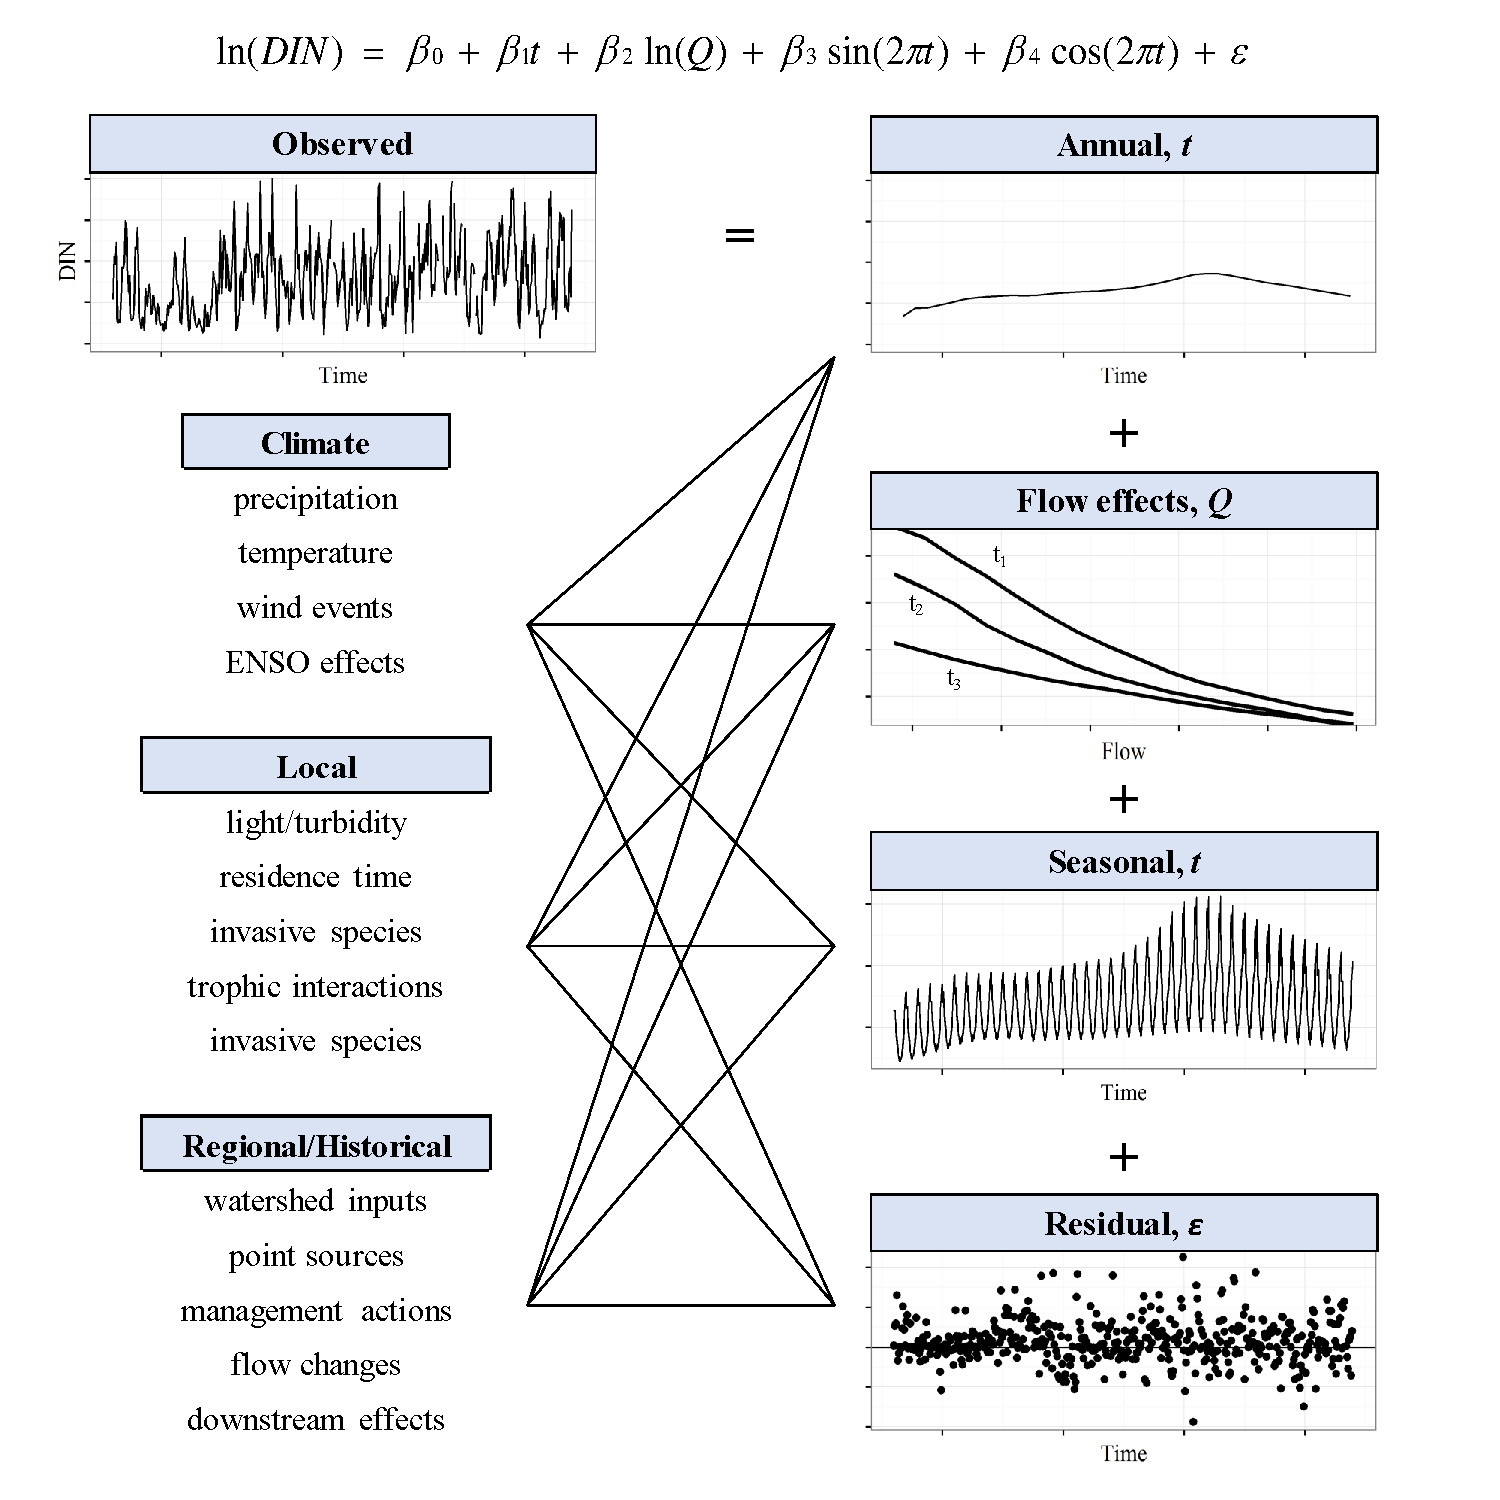
\includegraphics[width=1\textwidth,page=1]{figs/schematic.pdf}
\caption{Conceptual diagram illustrating use of \ac{wrtds} to decompose trends in observed nitrogen time series and potential forcing factors that can explain model output.  Results from the model are described as annual and seasonal trends, changes in flow-nutrient dynamics for different time periods, and residual variation independent of time, flow, and season. Relationships between environmental factors (climate, local, regional/historical) and nitrogen trends are more easily related to the separate components of the observed time series using results from the model. }
\label{fig:schematic}   
\end{figure}

\begin{figure}[!ht]

{\centering 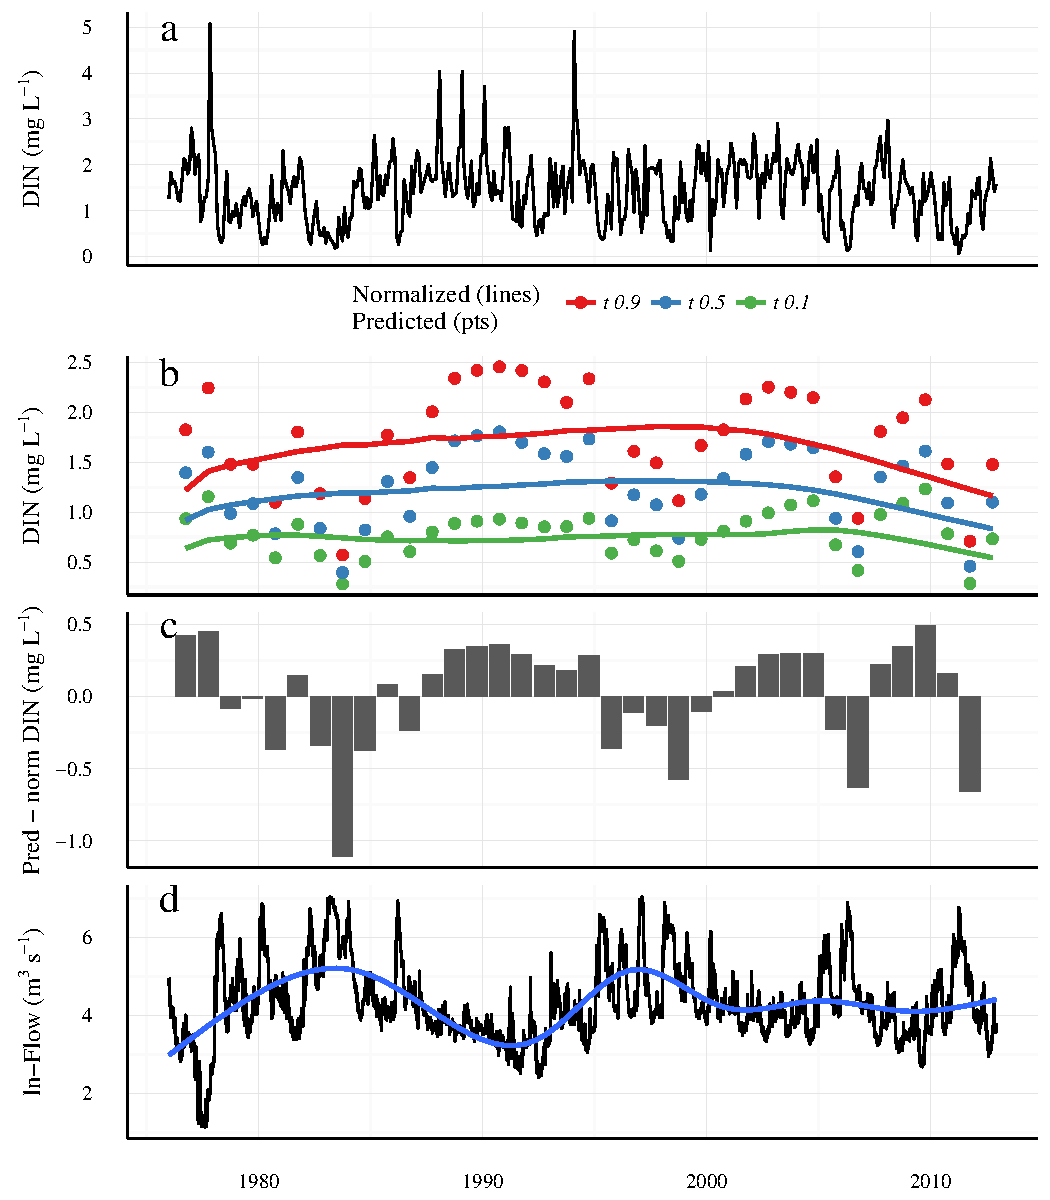
\includegraphics[width=0.75\textwidth]{figs/dinc10-1} 

}

\caption{Time series of \ac{din} and flow at station C10.  Subfigure (a) shows the observed \ac{din} time series and subfigure (b) shows the annual (water year starting in October) predictions from \ac{wrtds} at different conditional quantiles ($\tau$ = 0.1, 0.5, 0.9).  The points in subfigure (b) are predictions of observed \ac{din} and the lines are flow-normalized predictions.  Subfigure (c) shows the difference between the model predictions and flow-normalized predictions at the fiftieth conditional quantile.  Subfigure (d) shows the flow time series of the San Joaquin River with a locally-estimated (loess) smooth to emphasize the long-term trend.}\label{fig:dinc10}
\end{figure}



\begin{figure}[!ht]

{\centering 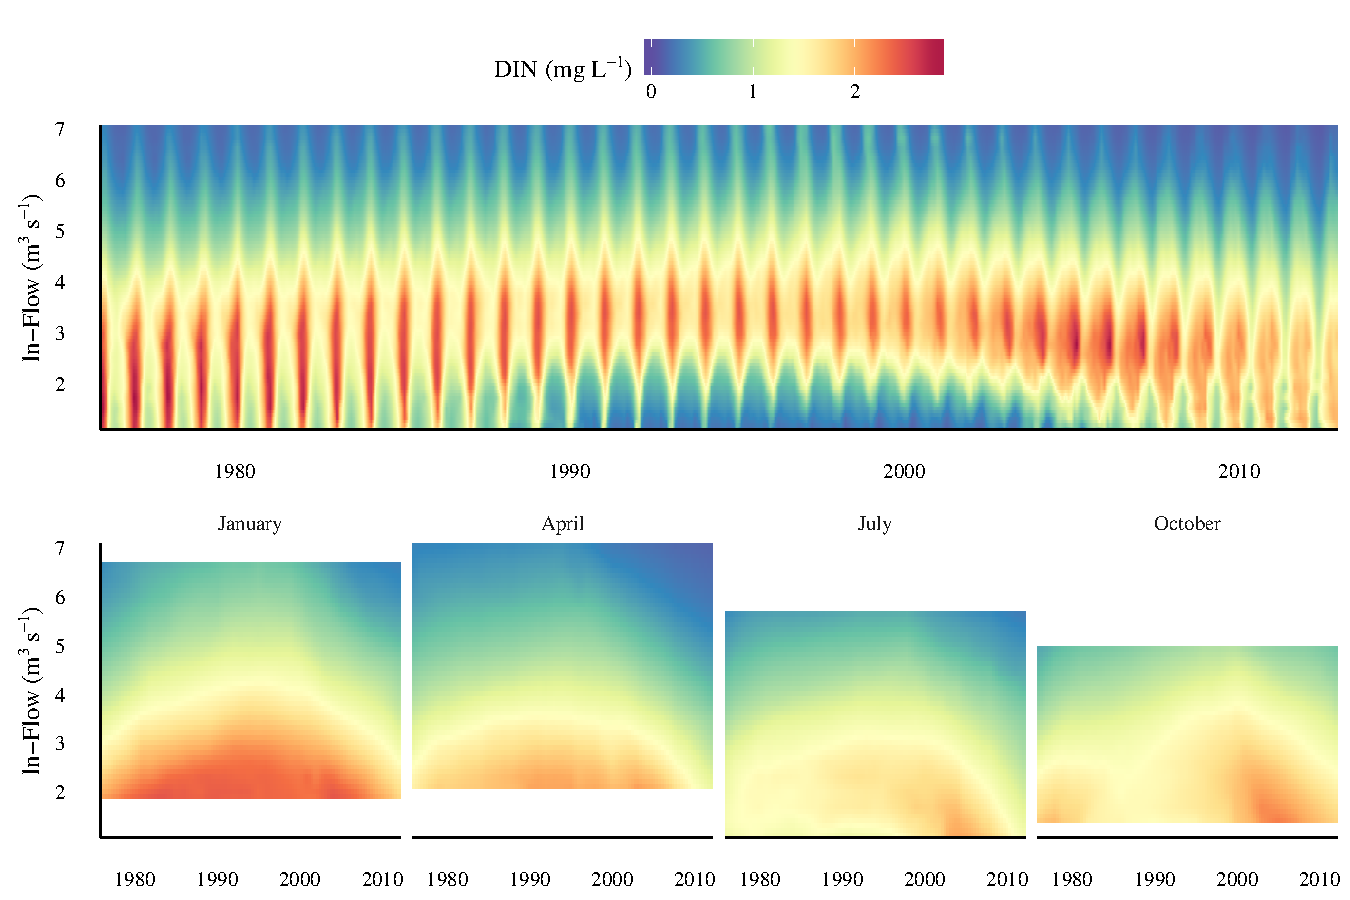
\includegraphics[width=\textwidth]{figs/dinc10dyna-1} 

}

\caption{Modelled relationships between \ac{din}, flow, and time at station C10.  The top figure shows the annual and seasonal variation over the entire time series and the bottom figure shows annual variation for selected months to remove seasonal variation.  Warmer colors indicate higher \ac{din} concentrations.  The y-axis on the bottom figure is truncated by the fifth and ninety-fifth percentiles of flow within each month.  Model results are for the fiftieth conditional quantile of \ac{din}.}\label{fig:dinc10dyna}
\end{figure}



\begin{figure}[!ht]

{\centering 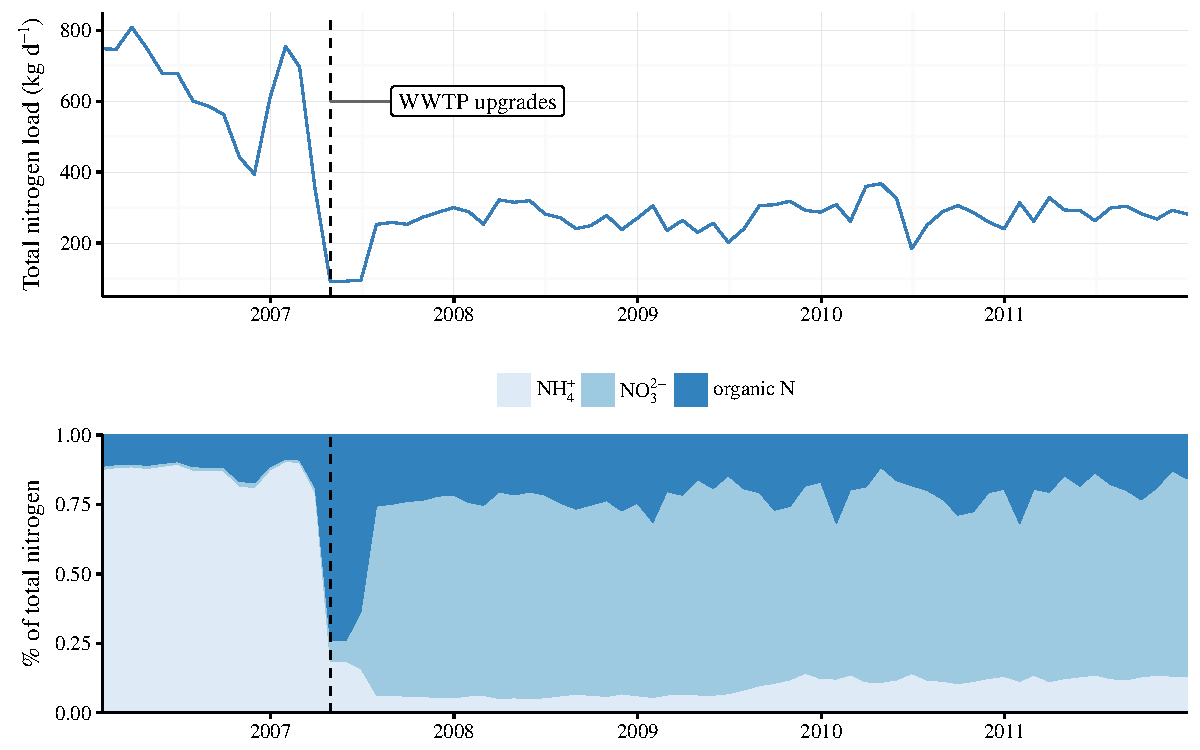
\includegraphics[width=\textwidth]{figs/tracy-1} 

}

\caption[Nitrogen load measurements (kg d]{Nitrogen load measurements (kg d$^{-1}$) at the City of Tracy Wastewater Treatment Plant, San Joaquin County.  Wastewater discharge requirements were implemented in May, 2007 to include nitrification/denitrification and tertiary filtration causing a reduction in total nitrogen effluent discharged to the Delta. Reductions were primarily observed for ammonium.}\label{fig:tracy}
\end{figure}



\begin{figure}[!ht]

{\centering 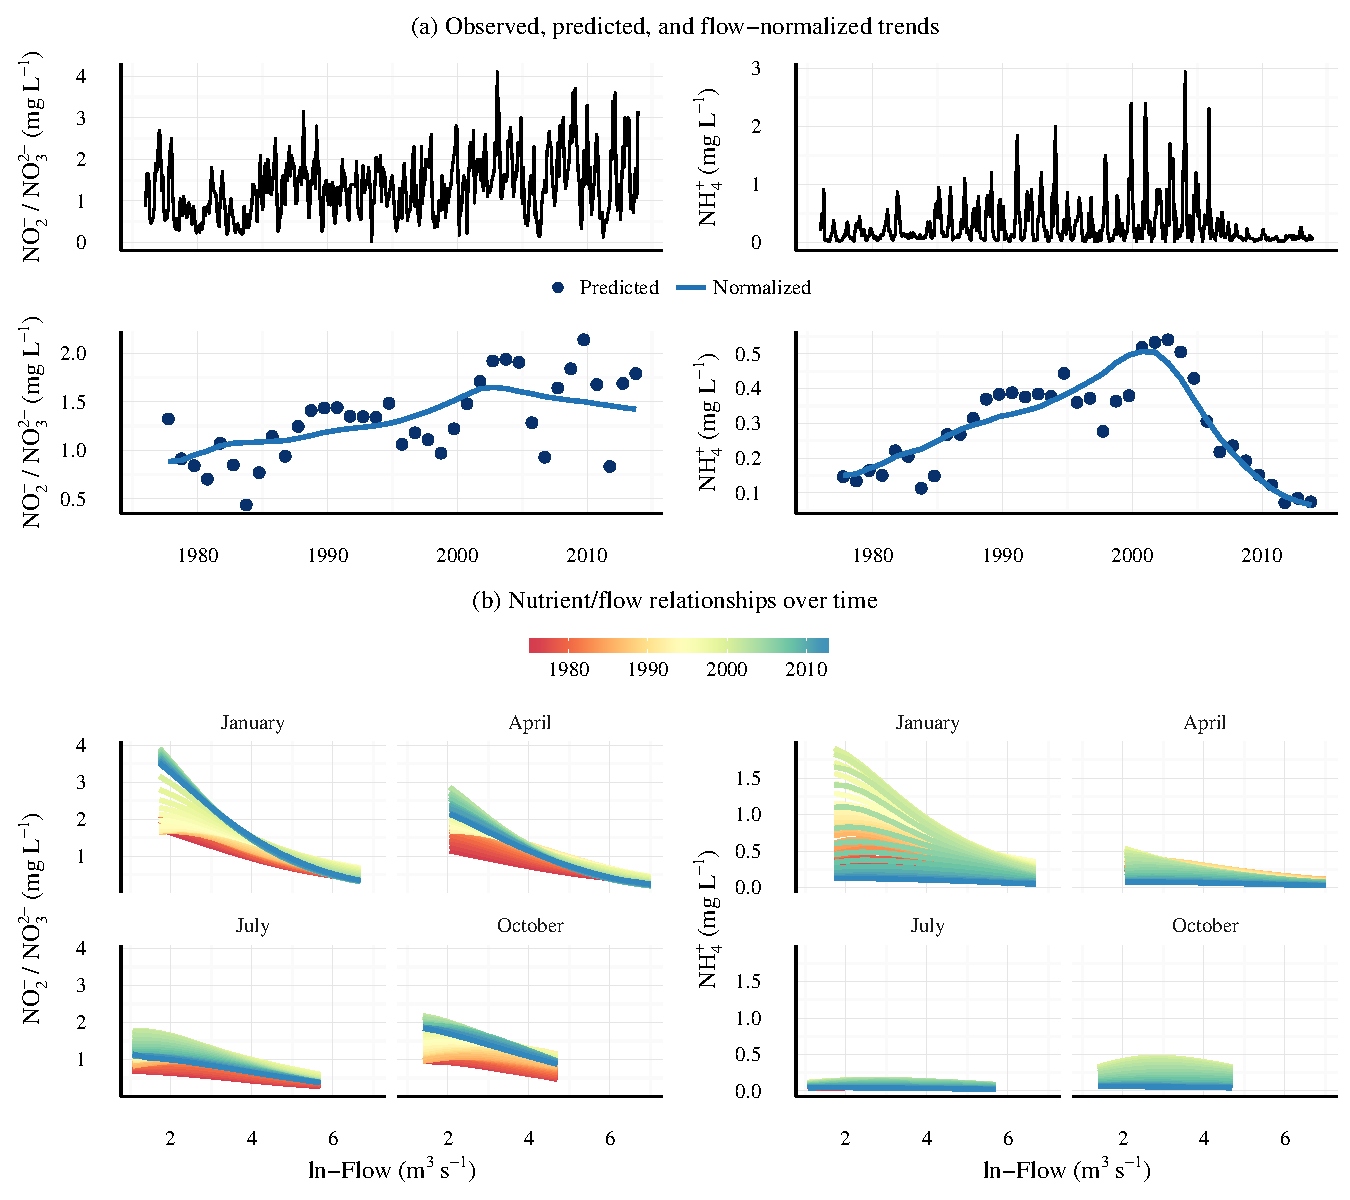
\includegraphics[width=\textwidth]{figs/p8trnds-1} 

}

\caption{Nitrogen trends at P8 as observed (a, top), predicted and flow-normalized estimates from \ac{wrtds} (a, bottom), and relationships with flow over time (b).  Nitrite/nitrate trends are on the left and ammonium trends are on the right.  Wastewater treatment plant upgrades at the City of Tracy (San Joaquin County), were completed in May 2007 (\cref{fig:tracy}), coincident with a dramatic decrease in ammonium at P8.}\label{fig:p8trnds}
\end{figure}



\begin{figure}[!ht]

{\centering 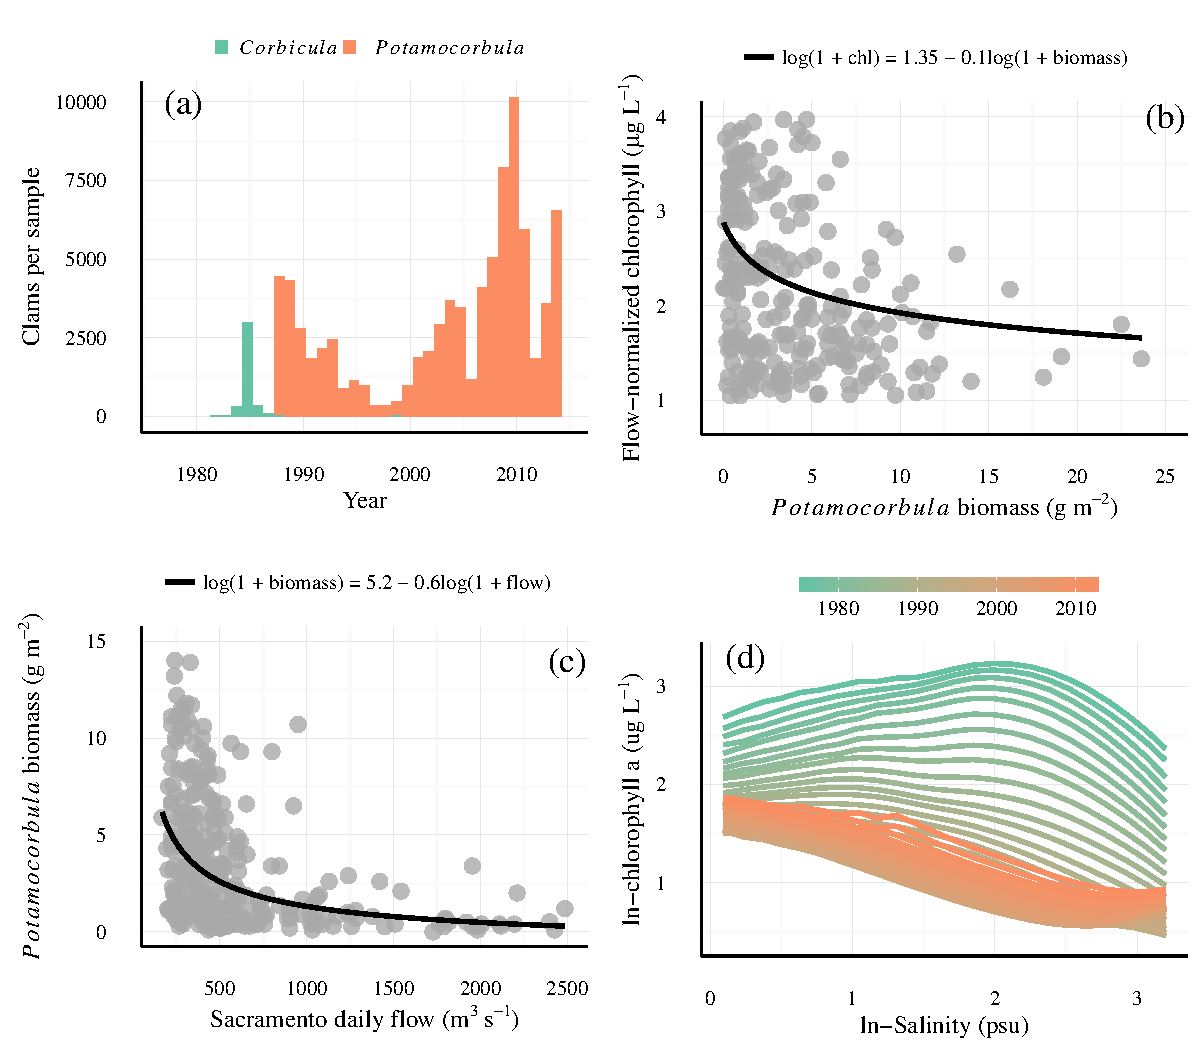
\includegraphics[width=\textwidth]{figs/clmchl-1} 

}

\caption{Trends in clam abundance and \ac{chla} concentration from 1976 to 2014 at station D7 in Suisun Bay.  Invasion by \textit{Potamocorbula amurensis} clams in the late 1980s and displacement of \textit{Corbicula fluminea} was shown by changes in clam density (a, annual means).  A coincident decrease in \ac{chla} concentration was also observed (c).  A weak but significant ($p < 0.001$) relationship between clam biomass and \ac{chla} concentration is shown in subfigure (b).  Flow relationships with \ac{chla} concentration have also changed over time (d, observations from June). Chlorophyll shows a slight positive then dominantly negative association with increasing flow (decreasing salinity) early in the time series, whereas the trend is reversed in recent years.}\label{fig:clmchl}
\end{figure}



\begin{figure}[!ht]

{\centering 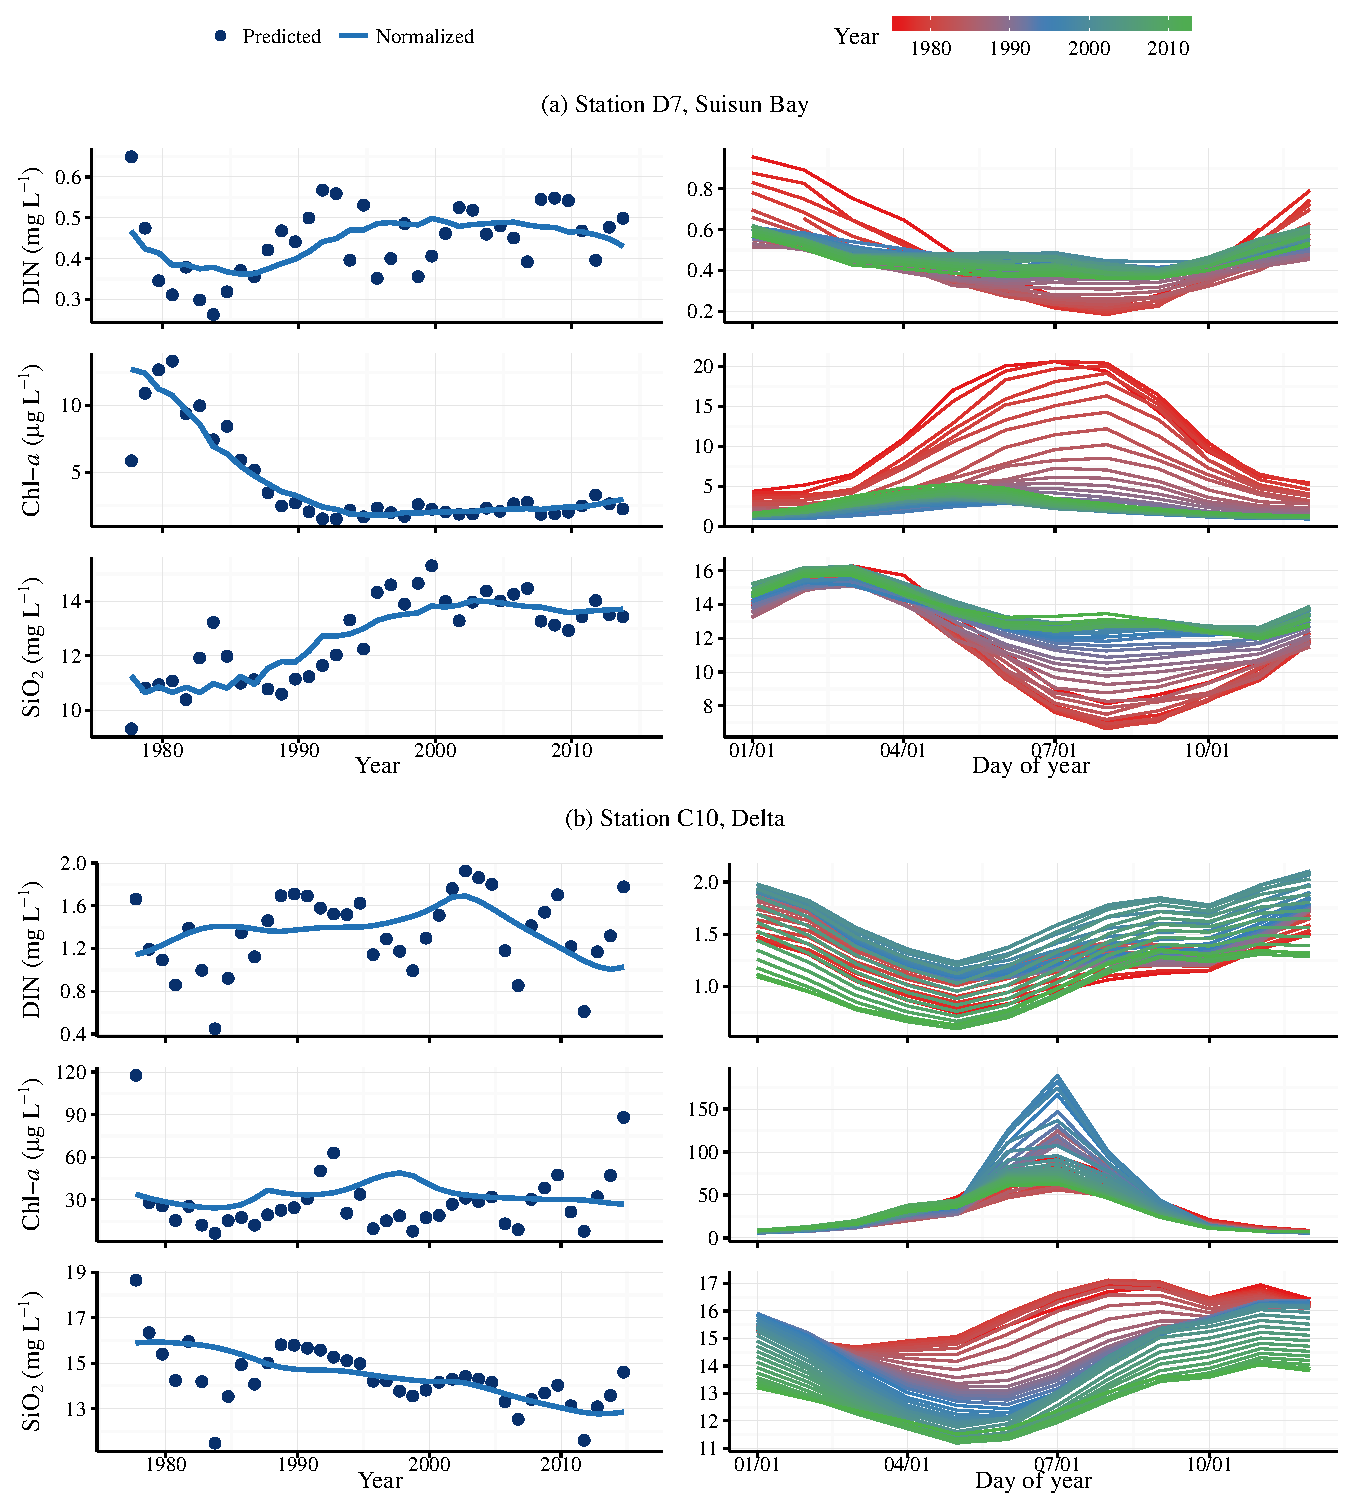
\includegraphics[width=\maxwidth]{figs/d7c10trnds-1} 

}

\caption{Flow-normalized trends of annual (left) and seasonal (right) variation in DIN, chl-{\it\footnotesize a}, and SiO$_2$ at station D7 (top) and C10 (bottom).  Covariation between nutrients, chl-{\it\footnotesize a}, and SiO$_2$ is observed at D7 but not C10, although an overall decrease in SiO$_2$ at C10 is shown.  Seasonal changes at D7 are most pronounced during the summer.}\label{fig:d7c10trnds}
\end{figure}



\clearpage
%%%%%%
% tables

% trends in din, chl, sio2 at d7
%latex.default(totab, file = "", rowlabel = "Period", caption = cap.val,     caption.loc = "top", rgroup = segs, n.rgroup = c(1, rep(4,         2)), cgroup = vars, n.cgroup = c(2, 2, 2), rowname = cats,     label = "tab:d7chg")%
\begin{table}[!tbp]
\caption{Summaries of flow-normalized trends in dissolved inorganic nitrogen (mg $L^{-1}$), chlorophyll ($\mu$g $L^{-1}$), and silicon dioxide (mg $L^{-1}$) concentrations for different time periods at station D7. Summaries are means and percent changes based on annual means within the time periods.  Increasing values are in bold-italics.\label{tab:d7chg}} 
\begin{center}
\begin{tabular}{lllcllcll}
\hline\hline
\multicolumn{1}{l}{\bfseries Period}&\multicolumn{2}{c}{\bfseries DIN}&\multicolumn{1}{c}{\bfseries }&\multicolumn{2}{c}{\bfseries Chl-\textit{a}}&\multicolumn{1}{c}{\bfseries }&\multicolumn{2}{c}{\bfseries SiO$_2$}\tabularnewline
\cline{2-3} \cline{5-6} \cline{8-9}
\multicolumn{1}{l}{}&\multicolumn{1}{c}{Mean}&\multicolumn{1}{c}{\% change}&\multicolumn{1}{c}{}&\multicolumn{1}{c}{Mean}&\multicolumn{1}{c}{\% change}&\multicolumn{1}{c}{}&\multicolumn{1}{c}{Mean}&\multicolumn{1}{c}{\% change}\tabularnewline
\hline
{\bfseries All}&&&&&&&&\tabularnewline
~~1976-2013&0.4&-4.2&&4.6&-82.4&&12.5&\textit{\textbf{30}}\tabularnewline
\hline
{\bfseries Annual}&&&&&&&&\tabularnewline
~~1976-1985&0.4&-15.2&&10.2&-67.9&&10.7&\textit{\textbf{8.4}}\tabularnewline
~~1986-1994&0.4&\textit{\textbf{15.4}}&&3.3&-48.8&&12.3&\textit{\textbf{13.5}}\tabularnewline
~~1995-2003&0.5&\textit{\textbf{4.3}}&&2.1&-3.9&&13.5&\textit{\textbf{3.7}}\tabularnewline
~~2004-2013&0.5&-10.6&&2.5&\textit{\textbf{31.7}}&&13.7&-1.8\tabularnewline
\hline
{\bfseries Seasonal}&&&&&&&&\tabularnewline
~~JFM&0.5&-4.9&&2.7&-56&&15&\textit{\textbf{4.4}}\tabularnewline
~~AMJ&0.4&\textit{\textbf{17.4}}&&6.1&-74.3&&12.9&\textit{\textbf{20.9}}\tabularnewline
~~JAS&0.3&\textit{\textbf{40.6}}&&6.2&-89&&10.9&\textit{\textbf{79.1}}\tabularnewline
~~OND&0.5&\textit{\textbf{13.1}}&&2.7&-83.8&&11.7&\textit{\textbf{33.7}}\tabularnewline
\hline
\end{tabular}\end{center}

\end{table}


% trends in din, chl, sio2 at c10
%latex.default(totab, file = "", rowlabel = "Period", caption = cap.val,     caption.loc = "top", rgroup = segs, n.rgroup = c(1, rep(4,         2)), cgroup = vars, n.cgroup = c(2, 2, 2), rowname = cats,     label = "tab:c10chg")%
\begin{table}[!tbp]
\caption{Summaries of flow-normalized trends in dissolved inorganic nitrogen (mg $L^{-1}$), chlorophyll ($\mu$g $L^{-1}$), and silicon dioxide (mg $L^{-1}$) concentrations for different time periods at station C10. Summaries are means and percent changes based on annual means within the time periods.  Increasing values are in bold-italics.\label{tab:c10chg}} 
\begin{center}
\begin{tabular}{lllcllcll}
\hline\hline
\multicolumn{1}{l}{\bfseries Period}&\multicolumn{2}{c}{\bfseries DIN}&\multicolumn{1}{c}{\bfseries }&\multicolumn{2}{c}{\bfseries Chl-\textit{a}}&\multicolumn{1}{c}{\bfseries }&\multicolumn{2}{c}{\bfseries SiO$_2$}\tabularnewline
\cline{2-3} \cline{5-6} \cline{8-9}
\multicolumn{1}{l}{}&\multicolumn{1}{c}{Mean}&\multicolumn{1}{c}{\% change}&\multicolumn{1}{c}{}&\multicolumn{1}{c}{Mean}&\multicolumn{1}{c}{\% change}&\multicolumn{1}{c}{}&\multicolumn{1}{c}{Mean}&\multicolumn{1}{c}{\% change}\tabularnewline
\hline
{\bfseries All}&&&&&&&&\tabularnewline
~~1976-2013&1.3&-16.9&&27.6&-4.9&&14.5&-23.1\tabularnewline
\hline
{\bfseries Annual}&&&&&&&&\tabularnewline
~~1976-1985&1.3&\textit{\textbf{16.6}}&&26.6&-20.5&&15.7&-5\tabularnewline
~~1986-1994&1.4&\textit{\textbf{6.6}}&&27.5&\textit{\textbf{23.7}}&&14.8&-3.9\tabularnewline
~~1995-2003&1.4&-1.1&&29.3&-15.2&&14.1&-5.1\tabularnewline
~~2004-2013&1.2&-32.6&&27.3&\textit{\textbf{11}}&&13&-9.6\tabularnewline
\hline
{\bfseries Seasonal}&&&&&&&&\tabularnewline
~~JFM&1.4&-20.5&&12&\textit{\textbf{14.8}}&&14.3&-16.9\tabularnewline
~~AMJ&1&-26.4&&43&\textit{\textbf{3.1}}&&13.1&-27.5\tabularnewline
~~JAS&1.3&-3.7&&46.6&-13.6&&14.8&-26.1\tabularnewline
~~OND&1.6&-6.8&&8.7&-18.5&&15.6&-16\tabularnewline
\hline
\end{tabular}\end{center}

\end{table}


\end{document}
